%pdflatex-../thesis.tex
% vim:spell spelllang=en_us

% Networking

Networking is essential part of cloud computing because it is not be possible to access any services without networking. Every service in cloud computing system is accessed via network. Network is usually also used for communication between virtual machines, migrations, storage access and for many other tasks.


% L1
First part of networking to think about is physical layer. Various Ethernet versions are used for physical layer in cloud data centers. There are many versions with different link bandwidth and wiring, but 1G and 10G with twisted pairs or optical fibers is used most widely. There were 100M called Fast Ethernet but it does not make sense to use this for server link today, because of it's limited bandwidth and almost similar price compared to 1G.

% server
It is common to insert two independent \Ac{NIC}s into every server and connect them into independent \Ac{ToR} switches, because it improves fault-tolerance. There is usually one more \Ac{NIC} for remote management and some additional cards if \Ac{SAN} is used. Remote management can be connected using detached cable or shared with any of network cards. Separate cable brings more flexibility and fault-tolerance and shared cable reduces cabling effort and thus simplifies maintenance and improves cooling effectiveness. Both solutions are used. 

% rack & ToR
About 40 servers fits into traditional rack and these serverl need to be connected to network infrastructure. There are different topologies, but most common is variant of two or three tier hierarchical structure. \cite{survey-architectures} There is also approach called \Uv{fabric} which implies non-blocking every-to-every mesh connection between switches. However fabric technologies are proprietary and limited to vendor. TODO: doplnit a více ocitovat surver-architectures

Every rack contains about 40 servers and these servers are connected to switch called \Ac{ToR}. This switch is located in the rack and acts as access layer for servers. Servers are connected to at least two \Ac{ToR}s if additional fault-tolerance is needed. Upper network topology layers depends on data center size and scaling requirements. There can be distribution and core layer, collapsed core or some kind of fabric.

Physical topology must be adjusted to spread network layers between two or more datacenter networks. It is obviously not possible to spread physical layer, but data link layer and upper layers are possible to spread.

% L3 & address
Another view on network topology is at network layer. Internet is based on \Ac{TCP}/\Ac{IP} so it is necessary to use this protocol family and assign \Ac{IP} addresses to servers, virtual machines and other network elements. There are two different versions of \Ac{IP} protocol:
\begin{description}
	\item[version 4] is the older one, with 32 bit address space. This version is still used more than version 6 even though it's address space is depleted and new version exists for more than 15 years.
	\item[version 6] is the \Uv{new} one, uses 128 bit address space and different headers, thus it is incompatible with version 4.
\end{description}

Moder data center must provide both versions of \Ac{IP} protocol, because supporting only one versions is a huge limitation and can not be accepted for new services deployment. 
However there is a problem with obtaining \Ac{IPv4} addresses, because available pool had already been depleted and all available addreses had been divided between \Ac{RIR}s. It is beneficial to make efforts to employ \Ac{IPv6} protocol as primary one and try to limit the amount of required \Ac{IPv4} addresses.


There are different ways how to use both versions concurently:
\begin{itemize}
	\item Dual-stack is the simpliest and probably the most used solution. Each interface gets at least one \Ac{IPv4} and one \Ac{IPv6} address. Use of both versions causes additional maintenance effort because it is necessary to take care of two separate L3 networks.
	\item Tunelling \Ac{IPv6} via existing \Ac{IPv4} infrastructure with technologies like 6to4, 6rd or \Ac{ISATAP} is another way. This solution can be used for \Ac{IPv6} deployment in networks with working \Ac{IPv4}, because it is used for transmission of all packets. 
	Tunelling is usually focused on deployment in access networks, but deployment in data center network is also applicable, as described in \cite{draft-sakura-6rd}.
	\item Translating \Ac{IPv4} addresses into part of \Ac{IPv6} addressing space is different approach than previous mentinoned, because it operates on \Ac{IPv6}-only networks. This technique does not require every box to have assigned an \Ac{IPv4} address and thus is good for saving address space. Hovewer address translations may not be suitable for data center usage, because it does not preserve original \Ac{IP} addresses and makes customer tracking almost impossible. Further information can be found in \cite{ipv4-jako-sluzba}.
\end{itemize}

It is beneficial to deploy protocol \Ac{IPv6} as primary one in my opinion, because it will become more and more needed during time. Hardware on current market usually support protocol \Ac{IPv6} at least partialy, but there are still some hidden pitfalls. There may be problem for example with server's remote management, because it may not support \Ac{IPv6} and thus is totally unusable on \Ac{IPv6}-only network. None of servers I have used for practical part of this thesis have support for \Ac{IPv6} on \Ac{IPMI}. 
However there is currently only small demand and \Ac{IPv6} deployment does not bring any direct profit. Even thought there are many problems and advantages are quite hidden, it is not possible to ignore this protocol and stay with old \Ac{IPv4}.

Virtual machine migration must be taken into account durring addressing schema design, because it plays crucial role in data center operation. Migrations are performed between hypervisors, i.e. physical servers, and these servers may be located in different racks, halls or even in different data centers. It is usually required to preserve \Ac{IP} address of virtual machine during migration process and thus adressing schema must be prepared to move single \Ac{IP} address around almost whole data center nwithout any significant configuration changes. 

% shared L2
First solution for unlimited migrations while preserving \Ac{IP} address is L2 sharing between hypervisors. Data link layer is shared between all hypervisors and then virtual machine is located in same L2 network before and after migration. This solution does not scale well since it is not recomended to place more than a few hundreds of hosts into single L2 domain, so it may be necessary to divide single big L2 into many smaller networks. It is quite easy to employ this solution for hypervisors in same rack, but it is more difficult with more distant servers and even more when servers are located at different data centers.

% routing 
Another way how to accomplish unlimited \Ac{VM} migrations is to use routinl for machine connectivity. This method uses temporary and fixed \Ac{IP} addresses. Hypervisor do not have to be in same L3 network and there is higher variability in addresses assigned to virtual machines. Temporary address is assigned according to \Ac{VM}'s location and it changes during migration. Fixed address is routed to \Ac{VM} and this address does not change, because changes are made only in routing tables. Any routing protocol can be usel, e.g. \Ac{OSPF}, to provide correct routing of fixed address destination virtual machine. Is is neccesary to insert one record in routing table for every virtual machine, because \textbackslash 32 routes are being advertised. Huge routing table may be problem for data centers with many virtual machines.
Higher layer is used to get more flexibility than lower level can offer. Main drawback of this solution is additinal complexity caused by routing and longer address swap, because it takes some time to propagate routing to new temporary address. It is not easy to perform live migration, because it is neccesary to change \Ac{IP} address of \Ac{VM}'s interface and thus open sessions will terminate.

\subsection{Overlays}
Virtualization is used heavily these days, therefore it is necessary provide networking solution with at least same flexibility as virtualization offers. Multitenancy, \Ac{VM} migrations, fast reconfiguration and rapid deployment are most missing features of physical networks these days. It is currently possible to migrate virtual machines without service interruption, but there is still not clear solution how to perform migration across whole data center with maintaining \Ac{IP} address. Overlay networking is one of proposed solutions and it is supposed to bring additional abstraction layer capable of decoupling network from physical hardware. 
Technologies capable to build overlay network are \Ac{VXLAN}, \Ac{STT} and \Ac{NVGRE}. 

% STP
Data center network need to be robust enough so parallel paths are used to provide redundancy and avoid outage caused by single link failure. It is necessary to avoid loops on L2 network because there are loops caused by redundant paths and L2 network does use anything like \Ac{TTL} field.  Spanning Tree Protocol (\Ac{STP}) can be used for avoiding loops in L2 networks, but there are two mayor problems. First is need to adjust \Ac{STP} if \Ac{VLAN}s are used because it is necessary to build special tree for each \Ac{VLAN}. Second problem with using \Ac{STP} is utilization of parallel links. \Ac{STP} keep only one of parallel link running and the others are disables to avoid topology loops. It is not optimal solution because links utilization is low and it is impossible to increase connection bandwidth by adding parallel links. Upgrading to higher link speed is limited and does not make economical sense. 10G cards are becoming affordable, but 40G cards are still expensive.

% MAC table at ToRs
Servers housed in rack are usually connected to switch called \Ac{ToR} and this switch is learning their \Ac{MAC} addresses. Common \Ac{ToR} switch have 24 or 48 ports so it should be able to learn addresses of these serves. However virtualization techniques let us to run many virtual machines on single physical server so number of \Ac{MAC} addresses can increase significantly. Amount of address may grow even more because each virtual machine can have more than one interface and \Ac{ToR} switch must be capable of learning all addresses.

% Tenant isolation
Public cloud solutions tend to serve many tenants and it is necessary to avoid unwanted interaction between them. It is quite easy to guarantee this on virtualization layer but much harder to accomplish on network layer. Tenant isolation can be performed on Layer 3 or Layer 2. \Ac{VLAN}s are often used for isolation on Layer 2, but this solution suffer from insufficient scaling issues because only 12 bit \Ac{VLAN} identifier is used and it provides only 4096 different tags. This might be enough for smaller solution but it is not sufficient for huge cloud system. Each physical server can host up to 100 virtual machines/containers\footnote{Server node2.brg/vpsfree.cz is currently running 117 \Ac{VPS}s with hardware: Supermicro \mbox{X9DR3-F}, 2x Xeon E5 2630Lv2, 256GB DDR3, 8x 2TB WD2002FAEX, 2x Intel DC S3700 200GB} owned by different tenants so 1 server can consume about 100 \Ac{VLAN} tags. All available tags can be depleted by 40 high performance servers which can fit in just one rack. Isolation at Layer 3 is does not provide sufficient scaling as well. It is necessary to provide unlimited migration facility between hypervisors in different racks and sometimes is required to spread Layer 2 between all tenant's virtual machines. Layer 3 isolation is not capable of this.


%Some kind of encapsulation is usually used to build overlay network on top of physical network. Encapsulation of course have drawbacks in higher computation demand and packet size problems, but advantages brought by overlay are appreciable:
%\begin{itemize}
%	\item Configuration of physical network is left untouched, so configuration fails are minimized
%	\item Overlay network is only virtual and more flexible than physical network
%	\item It is easy to adjust overlay network since it is only done in software
%	\item Tenant isolation can be done better because overlays are designed to support this
%\end{itemize}

\subsubsection{VXLAN}
Virtual eXtensible Local Area Network is an overlay scheme with multitenancy and domain isolation. It is defined on Layer 3 and uses encapsulation as tunneling mechanism.

Most important think is encapsulation since it provides \Ac{VXLAN} domain isolation and defines overlay network. Block called \Ac{VTEP} is responsible for encapsulation and tunnel organization. It analyzes every packet received from \Ac{VM} and prepend outer header with label. This label is called \Ac{VXLAN} Network Identifier (\Ac{VNI}) and it is used to isolate domains so virtual machines in different domains are not allowed to communicate directly with each other. Encapsulated packet is send to destination \Ac{VTEP} as \Ac{UDP} packet. Destination \Ac{VTEP} unpacks packet, check whether there is any virtual machine in \Ac{VXLAN} domain and deliver this frame. \Ac{NVE} is another term for \Ac{VTEP} and it was introduced in \cite{7365} as part of general network virtualization framework.

It is necessary for \Ac{VTEP} to be able to find destination \Ac{VTEP} for every encapsulated packet. This can be solved by data plane learning during forwarding as specified in \cite{rfc7348} or by acquiring this information from orchestrator. Getting information from orchestrator in my opinion much better because it avoids additional actions. Some kind of orchestrator or at least information system must be present in every data center and this system already knows location of all virtual machines as well as addresses of \Ac{VTEP}s. I think that it does not make sense to perform learning during forwarding because required informations are already saved in orchestrator. Orchestrator can directly distribute forwarding rules to all \Ac{VTEP}s or \Ac{VTEP} can ask orchestrator on-demand via any kind of \Ac{API}. Overlay unicast traffic can be forwarded directly to destination \Ac{VTEP} without any additional learning or even flooding.

% BUM traffic
There is traffic called \Ac{BUM} - Broadcast, Unknown unicast and Multicast which not easy to handle by \Ac{VXLAN}. This kind of traffic needs to be delivered to more than one host in a single \Ac{VXLAN} domain and thus it is necessary to send encapsulated packet to many \Ac{VTEP}s at the same time. Multicast should be used ad described in \cite{rfc7348}, but it needs mapping between \Ac{VXLAN} \Ac{VNI} and multicast address. This mapping should be managed by orchestrated by management layer. 
It would be beneficial to have technology for delivering \Ac{BUM} traffic without need of multicast because it brings additional complexity and it is not allowed in global Internet. Unknown unicast can be mitigated with getting information about addresses from orchestrator as described in previous paragraph because the orchestrator knows all addresses and there will no longer exists any unknown traffic. 
Sending encapsulated broadcast and multicast to many \Ac{VTEP}s can be achieved by multicast in underlay network or any advanced delivery methods can be uses. It is possible to send this traffic as unicast between source \Ac{VTEP} and every other \Ac{VTEP}. However this solution is suboptimal thanks to packet duplication and higher network bandwidth usage. Only one advantages is that multicast in underlay network is not required. It is also possible to select on node as \Uv{router} for encapsulated \Ac{VXLAN} traffic between \Ac{VTEP}s but it is technically similar to building multicast tree and thus it might be easier to deploy multicast in underlay.
There is proprietary technology called IBM DOVE with is very similar to \Ac{VXLAN} but does not require multicast.

% network requirements

% VXLAN conclusion
I think that\Ac{VXLAN} is quite promising technology for network virtualization in data center. It brings much more flexibility that traditional \Ac{VLAN} approach and it can be called as en evolution of \Ac{VLAN}. Principle of overlay network is building virtual network on top of physical infrastructure. Benefits were described in previous articles and main drawback is lack of cooperation between overlay and underlay network. Multicast might be also quite problematical to arrange.

\begin{figure}[htb]
	\begin{center}
	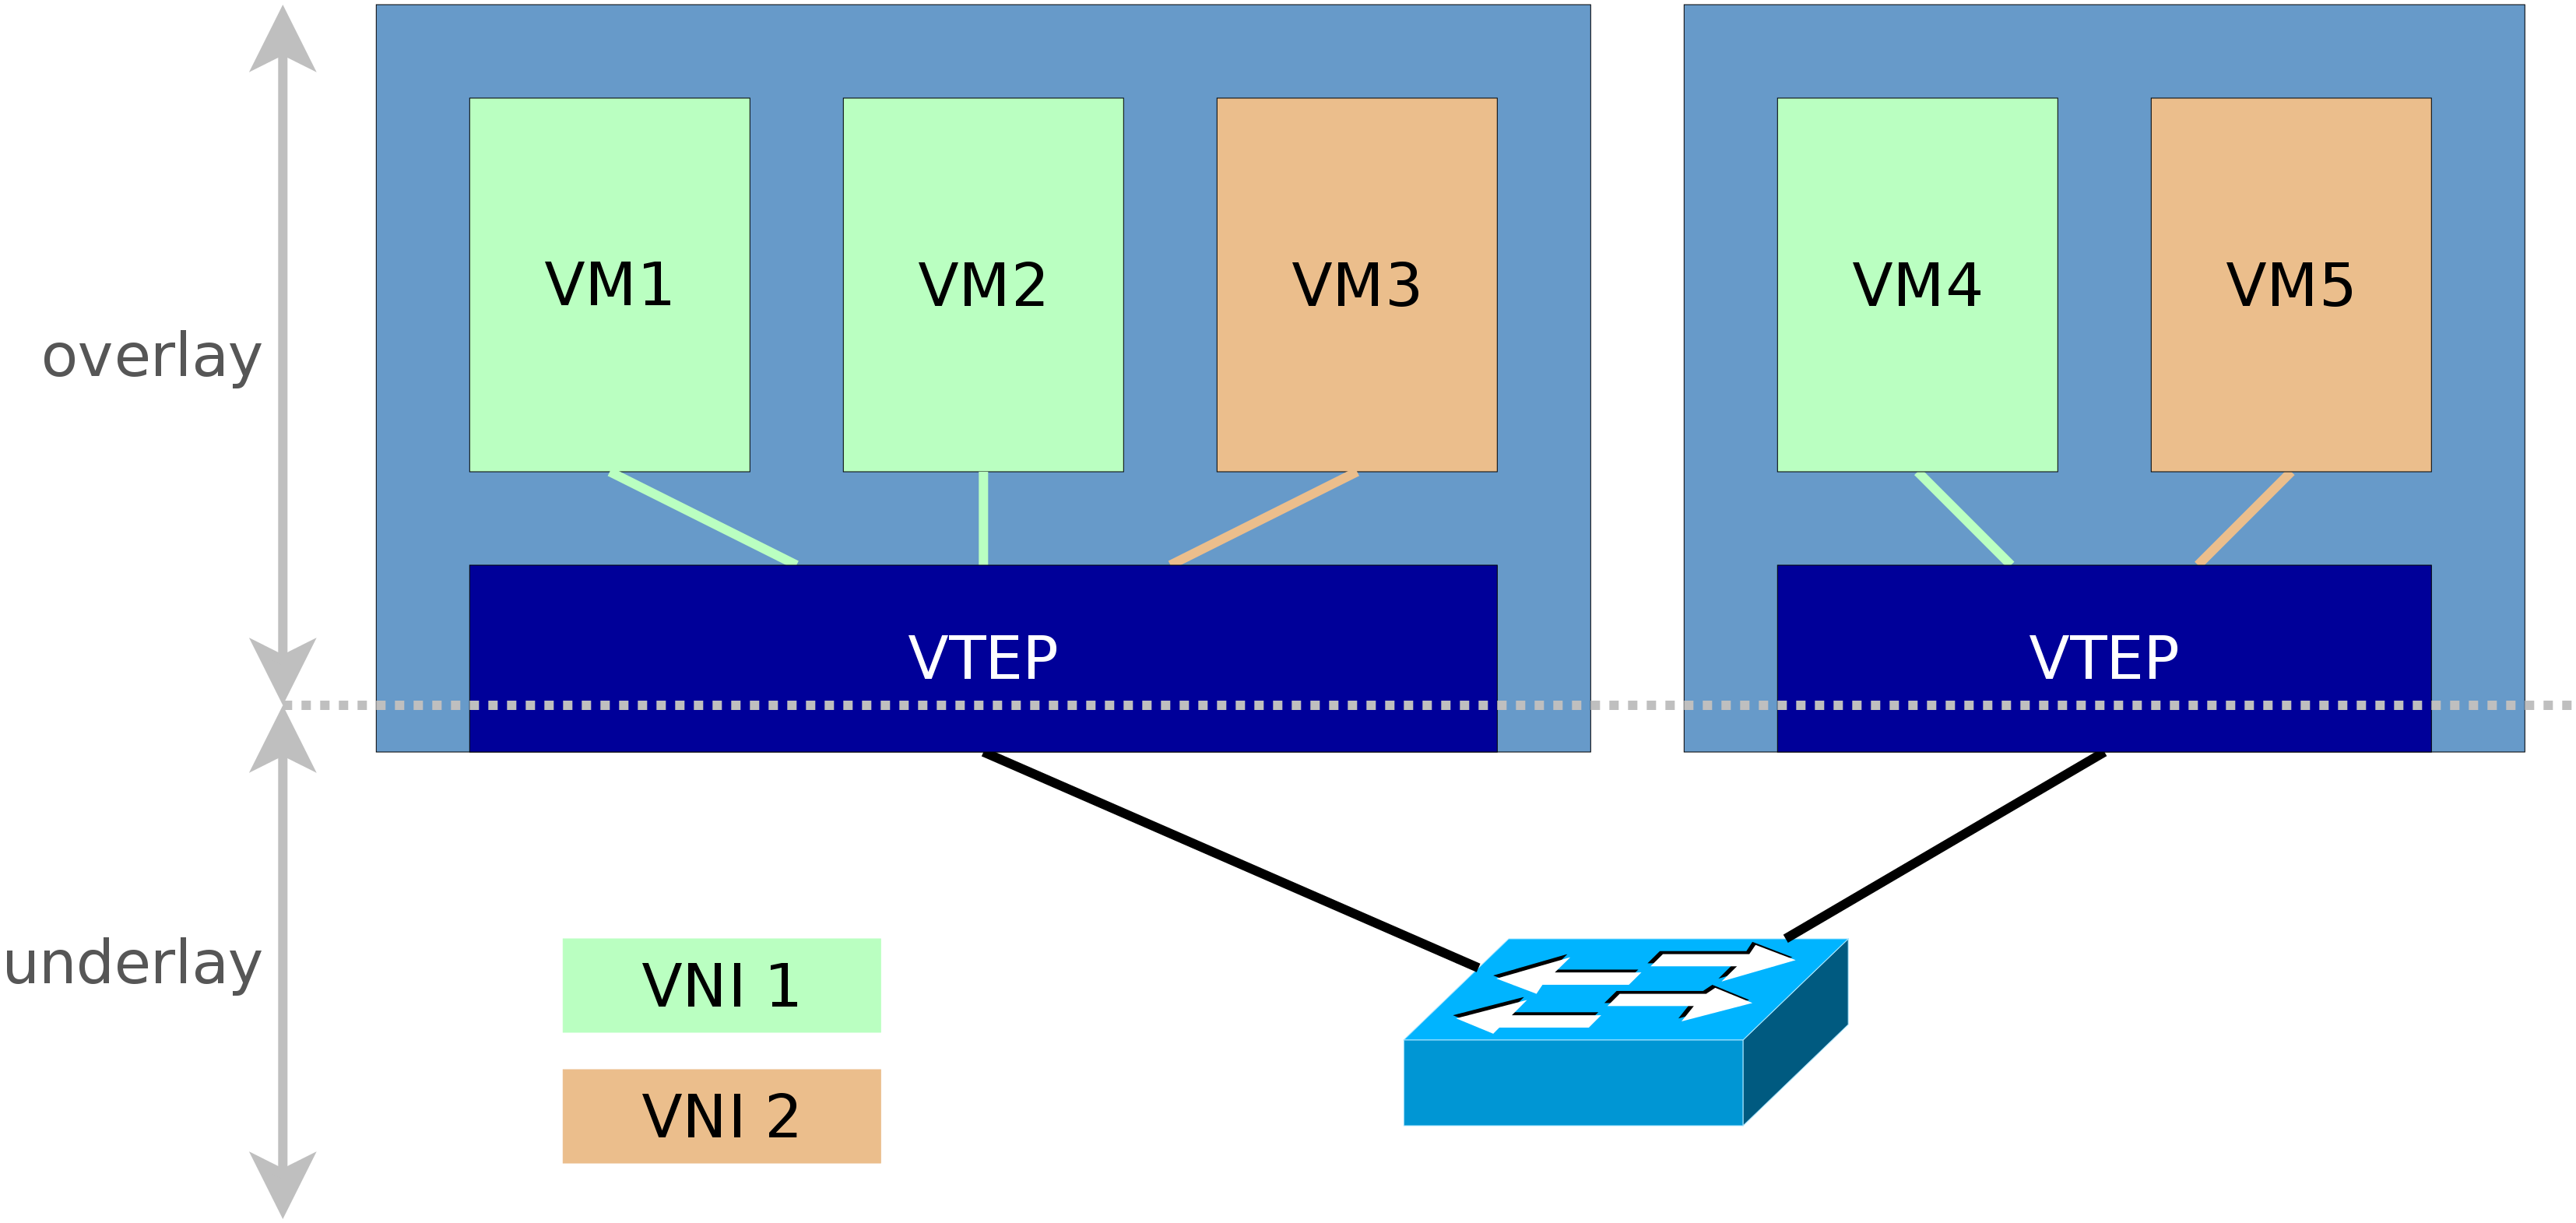
\includegraphics[width=0.9\textwidth]{vxlan.png}
	\end{center}
	\caption{Model of VXLAN topology}
	\label{img:vxlan-topology}
\end{figure}

\subsubsection{NVGRE}
Network virtualization using \Ac{GRE} is another overlay technology for multi-tenant data centers. It is very similar to previously mentioned \Ac{VXLAN} because it uses same topology scheme with different encapsulation mechanism. I am not going to provide detailed description of protocol as with \Ac{VXLAN} but main differences will be mentioned.

The biggest difference is encapsulation mechanism. \Ac{VXLAN} uses own approach but \Ac{NVGRE} uses \Ac{GRE} encapsulation.  Using quite old encapsulation standard may be beneficial because some boxes already support it and there is no need to make significant changes to physical infrastructure. Further information can be found in \cite{rfc2748} and \cite{rfc2890} describes header extensions used to carry \Ac{VSID}. \Ac{VSID} is identifier for virtual subnet isolation, it is analogue of \Ac{VNI} used by \Ac{VXLAN} with same length of $24~\Jed{b}$.

Outer header of packet with encapsulated payload is sent to destination \Ac{NVE} thus usage of \Ac{ECMP} may be suboptimal. There may be lack of entropy in outer header because destination address is same for all virtual machines residing at single \Ac{NVE}. This problem should be solved in \Ac{ECMP} hashing procedure by integrating \Ac{VSID} into sources for hash generation.


\subsubsection{STT}

\subsection{Storage network}
% storage network

\subsection{Load balancing}
% load balancing

\subsection{Firewall}
% firewall 

\subsection{Software Defined Networks}
